% \documentclass[../../Orator]{subfiles}
\documentclass[class={myRUCProject}, crop=false]{standalone}
\IfStandalone{%
    \import{../../}{customCommands}
    \import{../../}{INP-00-glossary}
    }{}

\begin{document}





The \gls{hh} model of \gls{ap} is a system of \gls{gls:nonlinear} differentiable equations with four state variables with respect to time, \(\unit{\V\membrane}\br{t}, \ n\br{t}, \ m\br{t}, \ h\br{t}\)~\cite{HodHux1952}. The model is built from approximating the characteristics of excitable cells, such as neurons, to a circuit-like construct \cref{fig:MembraneCircut}. 

Mathematically, the flow of current is represented as the change in voltage over time scaled by capacitance:
    \begin{equation}
       \capa \ode{\unit{\V}} = \curr\total \\
       \end{equation}
       and recall, \cref{eq:ionCurrent}, that the current through a given \gls{gls:ionChan} is the product of that channel's \gls{gls:contan} and the \gls{gls:rPote} for the specific ion
    \begin{equation}
        \curr\ion = {g_\bfm{ion}}(\unit{\V\membrane}-\unit{\V\ion})  
    \end{equation}
where \(\unit{\V\ion} = \equi\ion = \equi\reverse\). Thus, for a cell with \gls{Na} and \gls{K} channels, the total current through the the membrane can be defined by:
\begin{equation}
     \curr\total  =  \sum\ion^{i} I_i = \sum\ion^{i} \sbr{\cond_i \br{\unit{\V\membrane}-\unit{\V_i}}} 
\end{equation} 
with \(I\) representing the total membrane current per unit area; 
\begin{alignat}{5}
    &\quad \curr\total &&= \quad \curr\potassium \quad&&+ \quad \curr\potassium \quad&&+ \quad \curr\leakage \\ 
    \implies &\quad C\membrane \ode{\unit{\V\membrane}} &&=  \cond\potassium\br{\unit{\V\membrane} - \unit{\V\potassium}} &&+ \cond\sodium \br{\unit{\V\membrane} - \unit{\V\sodium}}  &&+ \cond\leakage \br{\unit{\V\membrane} - V_\rmm{L}} 
\end{alignat}
Where \(C\membrane\) the membrane capacitance per unit area; and \(\cond\potassium\), \(\unit{\V\potassium}\), along with  \(\cond\sodium\), \(\unit{\V\sodium}\) make up the \gls{gls:cond} and \gls{gls:rPote} of \gls{K} and \gls{Na} respectively.
The directly time dependent element of this equation is \(\unit{\V\membrane}\), with \(\cond\sodium\), and \(\cond\potassium\) dependent on both \(\br{\unit{\V\membrane}}\), and as described in \cref{sec:ap}, dependent on time as a consequence of \gls{gls:ionChan}.

Through long term experimentation, the duo of Hodgkin and Huxley divined a model built from the observations of smooth current change as a function of pores (or channels) that were either open or closed. By using a statistical approach, H\&H generated predictions for the probability of channels being open or closed at a given time in the process~\cite{HodHux1939}. 


H\&H presented the model as a set of four \glspl{ode} with respect to time.
\begin{sysEquation}[HodHuxSys]
    C\mm \ode{\unit{\V\membrane}} &= \mathrlap{I\mm - \sbr{\mcon\potassium n^4 \br{\unit{\V\membrane} - \unit{\V\potassium}} + \mcon\sodium m^3 h \br{\unit{\V\membrane} - \unit{\V\sodium}}  + \mcon\leakage \br{\unit{\V\membrane} - V_\rmm{L}}}}  && \\
    \ode{n} &=  \frac{n_\infty\br{\unit{\V\membrane}}-n}{\tau\nn\br{\unit{\V\membrane}}}  =\alpha\nn \br{\unit{\V\membrane}} \br{1-n} - \beta\nn \br{\unit{\V\membrane}} n \qquad&& \\
    \ode{m} &=  \frac{m_\infty\br{\unit{\V\membrane}}-m}{\tau\mm\br{\unit{\V\membrane}}}  =\alpha\mm \br{\unit{\V\membrane}} \br{1-m} - \beta\mm \br{\unit{\V\membrane}} m \qquad&& \\
    \ode{h} &=  \frac{h_\infty\br{\unit{\V\membrane}}-h}{\tau\hh\br{\unit{\V\membrane}}}  =\alpha\hh \br{\unit{\V\membrane}} \br{1-h} - \beta\hh \br{\unit{\V\membrane}} h \qquad &&
\end{sysEquation}

The `gating' variables \(m\) and \(h\), part \(n\) describe the time dependent kinetics of the voltage
The \gls{gls:ionChan} activation/inactivation\footnotemark~probabilities, denoted by \(\alpha_p, \, \beta_p : \, p \in \left\{n,m,h\right\}\), are defined such that:
\begin{align}
    \alpha_p\br{\unit{\V\membrane}} &= p_\infty \br{\unit{\V\membrane}} / \tau_p \\
    \beta_p\br{\unit{\V\membrane}}  &= \br{1 - p_\infty \br{\unit{\V\membrane}}} / \tau_p 
\end{align}
\begin{minipage}[c]{.5\textwidth}
    With \(p_\infty\) and its complementary probability \(\br{1-p_\infty}\) being the steady state values for activation and inactivation respectively~\cite{HodHux1952}. 
    In the original paper by Hodgkin and Huxley, the relationships of \(\alpha_p, \text{ and }\, \beta_p\) were defined
    % for squid axons by hodgkin and huxely
    as:
    \vfill
    \begin{align*}
    n &\implies \left\{
    \begin{aligned}
        \alpha\nn \br{\unit{\V\membrane}} &= 0.01 \, \cfrac{ 10 - V }{ \exp{ 10 - V } - 1} \\
        \beta\nn \br{\unit{\V\membrane}}  &= 0.125 \, \exp{-\cfrac{V}{80}} 
    \end{aligned} \right.
    \end{align*}
    Where \(\unit{\V} = \unit{\V_\rmm{rest}} - \unit{\V\membrane}\) represents the polarization in \unit{\milli\volt}
\end{minipage}
\hfill
\begin{minipage}[c]{.45\textwidth}
    \begin{align*}
    m &\implies \left\{
    \begin{aligned}
        \alpha\mm \br{\unit{\V\membrane}} &= 0.1 \cfrac{ 25 - V }{\exp{\cfrac{25-V}{10}} - 1} \\
        \beta\mm \br{\unit{\V\membrane}}  &= 4 \, \exp{-\cfrac{V}{18}} 
    \end{aligned} \right. \\
    h &\implies \left\{
    \begin{aligned}
        \alpha\hh \br{\unit{\V\membrane}} &=  0.07 \, \exp{-\cfrac{V}{20}} \\
        \beta\hh \br{\unit{\V\membrane}}  &= { \cfrac{1}{\exp{\cfrac{30 - V}{10}} + 1}}
    \end{aligned} \right.
    \end{align*}
\end{minipage}


\footnotetext{\underline{a}ctivation gives \(\alpha\), \underline{b}nactivation gives \(\beta\), really these are the obvious choices}

In order to characterize the ion-channels, the equations can be fitted to voltage clamp\footnotemark~data.
\footnotetext{An assay that measures the flow of current through a neuronal cell membrane by `clamping' the potential at an unchanging value.}

\begin{table}[htb]
    \centering
    \caption{Parameters of the \acrlong{hh} model determined from studies of squirts}\label{tab:my_label}
    \begin{tabular}{m{0.15\textwidth} @{}
                    p{0.55\textwidth}  @{}
                    m{0.15\textwidth}} \hline
        Parameters & Significations & Values \\\hline
    \(\curr\) & Membrane Current Density 0A/cm2 during space clamp & \\
    \unit{\capa\membrane} & Membrane Capacitance & 1 µF/cm2\\
    \unit{\V\membrane} & Membrane Potential & mV\\
    %t &time & ms\\
    \unit{\mcon\potassium} & maximal cond for \gls{K} & \qty{36}{m.mho/cm2} \\
    \unit{\mcon\sodium} & maximal cond for \gls{Na} &\qty{120}{m.mho/cm2} \\
    \unit{\mcon\leakage} & maximal cond for “leaking” ions & \qty{0.3}{\per\milli\ohm\per\square\cm} \\
    \unit{\V\potassium} & Resting Potential of \gls{K} & \qty{12}{mV} \\
    \unit{\V\sodium} & Resting potential for \gls{Na} & \qty{-115}{mV} \\
    \unit{\V\leakage} & Resting potential for “leaking” ions & \qty{-10.613}{mV} \\
    n & Proportion of particles in neuron involved with opening of \gls{K} gate & \\
    m & proportion of particles in neuron affecting opening of \gls{Na} gate & \\
    h & proportion of particles outside of neuron affecting closing of “2nd” \gls{Na} gate & \\
    \unit{\alpha\nn} & Voltage dependent rate for \gls{K} ions to enter the cell per ms & \\
    \unit{\beta\nn} & Voltage dependent rate for \gls{K} ions to exit the cell per ms & \\
    \unit{\alpha\mm} & Voltage dependent rate for \gls{Na} to enter the cell per ms via the “1st” gate & \\ 
    \unit{\beta\mm} & Voltage dependent rate for \gls{Na} to exit the cell per ms via the “1st” gate & \\
    \unit{\alpha\hh} & Voltage dependent rate for \gls{Na} to exit the cell per ms via the “2nd” gate & \\ 
    \unit{\beta\hh} & Voltage dependent rate for \gls{Na} to enter the cell per ms via the “2nd” gate &
    \end{tabular}
\end{table}

\begin{comment}
    Breaking down the equation we find the following regions:
    \begin{equation*}
        \curr = 
        \overbrace{C\mm \ode{\unit{\V\membrane}}}^{\mathclap{\text{rate of change of voltage scaled by capacitance}}} + 
        \mcon\potassium n^4 \br{\unit{\V\membrane} - \unit{\V\potassium}} + 
        \mcon\sodium m^3 h \br{\unit{\V\membrane} - \unit{\V\sodium}}  + 
        \mcon\leakage \br{\unit{\V\membrane} - V_\rmm{L}} 
    \end{equation*}




    \begin{figure}[h]
        \centering
        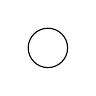
\begin{tikzpicture}
            
            \draw (0,0) circle (0.25);
            
        \end{tikzpicture}
        \caption{fart}\label{<label>}
    \end{figure}
\end{comment}



\end{document}
